% Copyright 2015 by Fabien Lahoudere <fabienlahoudere.pro@gmail.com>.
% !TEX TS-program = pdflatex
% !TEX encoding = UTF-8 Unicode

\documentclass{beamer}

\mode<presentation>
{
  \usetheme{Warsaw}
  \setbeamercovered{transparent}
}

\usepackage[english]{babel}
\usepackage[utf8]{inputenc}
\usepackage{times}
\usepackage[T1]{fontenc}
\usepackage{listingsutf8}

\definecolor{light-gray}{gray}{0.95}
\definecolor{light-blue}{RGB}{20,20,80}
\lstdefinestyle{customc}{language=C,
	breaklines=true,
	frame=L,
	xleftmargin=\parindent,
	showstringspaces=false,
	numbersep=5pt,
	tabsize=8,
	backgroundcolor=\color{light-gray},
	frame=shadowbox,
	rulesepcolor=\color{blue!40!white},
	basicstyle=\ttfamily\tiny,
	numberstyle=\tiny,
    keywordstyle=\bfseries\color{green!40!black},
    commentstyle=\itshape\color{purple!40!black},
    identifierstyle=\color{blue},
    stringstyle=\selectfont\color{orange}}

\lstdefinestyle{customshell}{language=bash,
	belowcaptionskip=1\baselineskip,
	basicstyle=\ttfamily\tiny}


\title[Debug Linux embarqué]
{Panorama des outils de debug pour Linux embarqué}

\author[Fabien Lahoudère]
{Fabien Lahoudère}

\institute[Open Wide]
{
  Développeur Linux embarqué chez Open Wide\\
  fabienlahoudere.pro@gmail.com\\
  aragua sur github et IRC
}

\date[Mai 2015]
{Toulouse Embedded Linux and Android Meetup, Mai 2015}

\subject{Debug Linux embarqué}

\AtBeginSubsection[]
{
  \begin{frame}<beamer>{Plan}
    \tableofcontents[currentsection,currentsubsection]
  \end{frame}
}


%%%%%%%%%%%%%%%%%%%%%%%    DOCUMENT    %%%%%%%%%%%%%%%%%%%%%%%
\begin{document}

\begin{frame}
  \titlepage
\end{frame}

\begin{frame}{Plan}
  \tableofcontents
\end{frame}

%%%%%%%%%%%%%%%%%%%%%%%    BUGS    %%%%%%%%%%%%%%%%%%%%%%%
\section{Bugs et erreurs}

\subsection{Définition}

\begin{frame}{Définition}{Qu'est ce qu'un bug?}
	\begin{itemize}
		\item
			Un défaut de conception d'un programme informatique à l'origine d'un dysfonctionnement.
		\item
			Gravité : défauts d’affichage mineurs -> crash système critique (explosion du vol 501 d'Ariane 5).
		\item
			Un bug peut résider dans n'importe quel logiciel contenant du code (application, librairie, firmware, ...)
	\end{itemize}	
\end{frame}

\begin{frame}{Définition}{Classification des cas courants}
	Exemple de classification des cas courants de bugs:
	\begin{itemize}
		\item
			Erreur de segmentation
		\item
			Dépassement d'entier
		\item
			Dépassement de tampon
		\item
			Dépassement de pile
		\item
			Fuite mémoire
		\item
			Situation de compétition
		\item
			Interblocage
		\pause
		\item
			Performance dégradée
	\end{itemize}
\end{frame}

\begin{frame}{Définition}{Les erreurs}
	\begin{itemize}
		\item
			Une erreur retournée par un programme n'est pas un bug.
		\item
			C'est une fonctionnalité permettant de notifier l'utilisateur d'un comportement anormal d'un logiciel. 
		\item
			Elle peut résulter d'un mauvais paramètre d'entrée ou d'un bug logiciel.
		\item
			Plusieurs types d'erreurs rencontrés par le développeur:
			\begin{itemize}
				\item
					Erreur de compilation
				\item
					Erreur système
				\item
					Erreur de l'application (gestion des bugs)
			\end{itemize}
	\end{itemize}
\end{frame}


\subsection{Exemple}

%%%%%%  segfault  %%%%%%
\defverbatim[colored]\mycode{%
\begin{lstlisting}[style=customc]
int main (int argc, char ** argv)
{
	char ptr[10];
	memcpy(ptr, argv[1], strlen(argv[1])+1);
	printf("%s\n", ptr);
	return 0;
}
\end{lstlisting}}

\defverbatim[colored]\myshell{%
\begin{lstlisting}[style=customshell]
$ ./segfault toto
toto
$ ./segfault
Erreur de segmentation (core dumped)
$
\end{lstlisting}}

\begin{frame}[fragile]{Erreur de segmentation}
Tentative d'accès à un segment de mémoire inexistant ou non autorisé.
\mycode
\myshell
\end{frame}


%%%%%%  Dépassement d'entier  %%%%%%
\defverbatim[colored]\mycode{%
\begin{lstlisting}[style=customc]
int main (int argc, char ** argv)
{
	short s;
	for(s=0; s < atoi(argv[1]); s++) {
	}
	printf("Succeed to count until %d\n", s);
	return 0;
}
\end{lstlisting}}
\defverbatim[colored]\myshell{%
\begin{lstlisting}[style=customshell]
$ ./intoverflow 32767
Succeed to count until 32767
$ ./intoverflow 32768
^C (infinite loop)
$
\end{lstlisting}}
\begin{frame}{Dépassement d'entier}
Un dépassement d'entier (integer overflow) est une condition qui se produit lorsqu'une opération mathématique produit une valeur numérique supérieure à celle représentable dans l'espace de stockage disponible.
\mycode
\myshell
\end{frame}


%%%%%%  Dépassement de tampon  %%%%%%
\defverbatim[colored]\mycode{%
\begin{lstlisting}[style=customc]
int main (int argc, char ** argv)
{
	char *buf2 = malloc(16), *buf1 = malloc(16);
	memcpy(buf1, argv[1], strlen(argv[1])+1);
	memcpy(buf2, argv[2], strlen(argv[2])+1);
	printf("%s\n", buf1);
	return 0;
}
\end{lstlisting}}
\defverbatim[colored]\myshell{%
\begin{lstlisting}[style=customshell]
$ ./bufoverflow hello abcdefghijklmnopqrstuvwxyz
hello
$ ./bufoverflow hello abcdefghijklmnopqrstuvwxyzabcdefghijklmnopqrstuvwxyz
ghijklmnopqrstuvwxyz
$
\end{lstlisting}}
\begin{frame}{Dépassement de tampon}
Un dépassement de tampon (buffer overflow) est un bug par lequel un processus, lors de l'écriture dans un tampon, écrit à l'extérieur de l'espace alloué au tampon, écrasant ainsi des informations nécessaires au processus.
\mycode
\myshell
\end{frame}


%%%%%%  Dépassement de pile  %%%%%%
\defverbatim[colored]\mycode{%
\begin{lstlisting}[style=customc]
int main (int argc, char ** argv)
{
	int idx=0; char buf[16];
	for(idx=0; idx <= strlen(argv[1]); idx++) {
		buf[idx]=argv[1][idx];
	}
	printf("read %d/%lu bytes\n%s\n", idx, strlen(argv[1])+1, buf);
	return 0;
}
\end{lstlisting}}
\defverbatim[colored]\myshell{%
\begin{lstlisting}[style=customshell]
$ ./stackoverflow 0123456789abcdefghijklmnopq
Read 28/28 bytes : 0123456789abcdefghijklmnopq
$ ./stackoverflow 0123456789abcdefghijklmnopqr
^C (infinite loop)
$ ./stackoverflow 0123456789abcdefghijklmnopqrs
Read 116/30 bytes : 0123456789abcdefghijklmnopqrt
$
\end{lstlisting}}
\begin{frame}{Dépassement de pile}
Un dépassement de pile (stack overflow) est un bug causé par un processus qui, lors de l'écriture dans une pile, va écraser les données précédemment pousser sur la stack.
\mycode
\myshell
\end{frame}


%%%%%%  Fuite mémoire  %%%%%%
\defverbatim[colored]\mycode{%
\begin{lstlisting}[style=customc]
int main (int argc, char ** argv)
{
	int size = atoi(argv[1]);
	while (1) {
		char * ptr = malloc(size);
		if (!ptr) // quit
			break;
		else // fill the buffer
			for(idx=0; idx < size ; idx++)
				ptr[idx]=idx;
	}
	return 0;
}
\end{lstlisting}}
\defverbatim[colored]\myshell{%
\begin{lstlisting}[style=customshell]
$ ./leak 12000000 &
$ watch cat /proc/meminfo 
...
MemFree:	xxxxxx kB # decrease until the system exit or start to swap
...
$
\end{lstlisting}}
\begin{frame}{Fuite mémoire}
Une fuite de mémoire est une occupation croissante et non contrôlée ou non désirée de la mémoire d'un ordinateur.
\mycode
\myshell
\end{frame}

%%%%%%  Situation de compétition  %%%%%%
\begin{frame}{Situation de compétition}
	\begin{itemize}
		\item
			Lorsque l'ordre d'utilisation d'une ressource partagée joue sur le résultat
		\item
			Par ex:
			\begin{itemize}
				\item
					Une variable est lue par un acteur avant d'être pourvue par un autre.
				\item
					Une fonction d'un système est exécuté avant que le système soit initialisé
			\end{itemize}
	\end{itemize}
\end{frame}

%%%%%%  Interblocage  %%%%%%
\begin{frame}{Interblocage}
	\begin{itemize}
		\item
			Lorsque un acteur détient un verrou et attend un signal d'un autre acteur attendant ce même verrou
		\item
			Plusieurs causes:
			\begin{itemize}
			\item
				Oubli de libérer le verrou
			\item
				Situation de compétition impliquant un verrou
			\item
				Mauvaise gestion des priorités entre threads
		\end{itemize}
	\end{itemize}
\end{frame}


%%%%%%%%%%%%%%%%%%%%%%%    TOOLS    %%%%%%%%%%%%%%%%%%%%%%%
\section{Les outils de debug pour Linux}

\subsection{Présentation des outils en espace utilisateur}

\begin{frame}{Printf et logs}
Intérêts:
\begin{itemize}
	\item
		Permet de montrer visuellement le bon fonctionnement d'un programme.
	\item
		Facilite l'identification d'erreur en environnement de production (sans moyen de debug)
	\item
		Facile à utiliser et mettre en place.
	\item
		Les logs permettent de garder des traces.
\end{itemize}
Inconvénients:
\begin{itemize}
	\item
		Joue sur la chronologie des événements.
	\item
		La modification nécessite une recompilation.
\end{itemize}
\end{frame}

\begin{frame}{Ptrace}
\begin{itemize}
	\item
		Ptrace est un appel système du noyau linux.
	\item
		Il permet à un processus en espace utilisateur de :
		\begin{itemize}
			\item
				contrôler l’exécution d'un autre processus
			\item
				accéder à l'espace mémoire d'un autre processus
			\item
				observer les appels systèmes d'un autre processus
		\end{itemize}
	\item
		Outils : strace, ltrace, gdb/gdbserver
	\item
		Pas à pas => pas de recompilation (ajout des symboles de debug)
\end{itemize}
\end{frame}

\begin{frame}{Ptrace}{gdb}
	\begin{itemize}
		\item
			Deux modes:
			\begin{itemize}
				\item
					local (gdb)
				\item
					distant (gdb + gdbserver)
			\end{itemize}
		\item
			Contrôle de l’exécution
		\item
			Accès mémoire, registres, threads, code source ...
		\item
			Analyse post-mortem (core)
		\item
			Activation des symboles de debug via l'option -g de gcc
		\item
			Intégré dans de nombreux IDE.
	\end{itemize}
\end{frame}


%% local
\defverbatim[colored]\gdblocal{%
\begin{lstlisting}[style=customshell]
$ gdb ./segfault
...
(gdb) b main
Breakpoint 1 at 0x4005c5: file segfault.c, line 8.
(gdb) r
Starting program: /.../segfault 

Breakpoint 1, main (argc=1, argv=0x7fffffffe2b8) at segfault.c:8
8		memcpy(ptr, argv[1], strlen(argv[1])+1);
(gdb) 
\end{lstlisting}}
\begin{frame}{Ptrace}{gdb local}
Démarrage gdb en local
\gdblocal
\end{frame}


%% remote
\defverbatim[colored]\gdbremote{%
\begin{lstlisting}[style=customshell]
$ gdbserver :9999 ./segfault
Process segfault created; pid = 12810
\end{lstlisting}}
\defverbatim[colored]\gdblocal{%
\begin{lstlisting}[style=customshell]
$ gdb myprog # gdb for the target architecture
GNU gdb (Sourcery CodeBench Lite 2012.03-57)
(gdb) target remote 192.168.2.2:9999
(gdb) set sysroot /.../rootfs_rpi
(gdb) b main
Breakpoint 1 at 0x4005c5: file segfault.c, line 8.
(gdb) c
\end{lstlisting}}
\begin{frame}{Ptrace}{gdb remote}
Démarrer gdbserver sur la target
\gdbremote
Lancer gdb sur le PC
\gdblocal
\end{frame}

\begin{frame}{Ptrace}{commandes gdb}
	\begin{itemize}
		\item
			break ou b : placer un breakpoint à une adresse
		\item
			run, next, step, continue : contrôler l’exécution
		\item
			backtrace, up, down : pour afficher la liste des fonctions appelantes et se déplacer dedans
		\item
			print : pour afficher une variable ou le contenu d'un registre
		\item
			x : affiche le contenu à une adresse
		\item
			display ajoute une commande à afficher à chaque arrêt
		\item
			info: donne des infos sur l'état du processus (threads, registres, ...)
		\item
			list : affiche le code source courant
	\end{itemize}
\end{frame}

\begin{frame}{Ptrace}{strace/ltrace}
	\begin{itemize}
		\item
			Trace des appels systèmes et bibliothèques
		\item
			Rustique mais efficace
		\item
			Filtrage des symboles à surveiller
		\item
			Possibilité de trier les résultats par pid  
	\end{itemize}
\end{frame}

\defverbatim[colored]\coredump{%
\begin{lstlisting}[style=customshell]
$ ulimit -c unlimited
$ ./segfault 
Erreur de segmentation (core dumped)
$ gdb ./segfault core
...
Core was generated by `./segfault'.
Program terminated with signal SIGSEGV, Segmentation fault.
#0  strlen () at ../sysdeps/x86_64/strlen.S:106
106	../sysdeps/x86_64/strlen.S: Aucun fichier ou dossier de ce type.
(gdb) bt
#0  strlen () at ../sysdeps/x86_64/strlen.S:106
#1  0x000000000040067f in main (argc=1, argv=0x7ffec66e7e68) at segfault.c:8
(gdb) up
#1  0x000000000040067f in main (argc=1, argv=0x7ffec66e7e68) at segfault.c:8
8		memcpy(ptr, argv[1], strlen(argv[1])+1);
(gdb) p argv[1]
$1 = 0x0
(gdb) list
3	
4	int main (int argc, char ** argv)
5	{
6		char ptr[10];
7	
8		memcpy(ptr, argv[1], strlen(argv[1])+1);
9		printf("%s\n", ptr);
10	
11		return 0;
12	}
(gdb)
\end{lstlisting}}
\begin{frame}[allowframebreaks]{Core dump}{Analyse post mortem avec gdb}
	\begin{itemize}
		\item
			Fonction du kernel : Userspace binary formats -> Enable core dump support		
		\item
			Au moment du crash, le noyau enregistre l'état du processus sous format binaire (fichier core)
		\item
			Utile en production pour remonter les crashs ou pour les bugs difficilement reproductible
		\item
			Ce fichier est lisible par gdb qui se met dans l'état au moment du crash
		\item
			L’exécution est figé mais on peut inspecter mémoire, variables, registres, ...
		\coredump			
	\end{itemize}
\end{frame}

\begin{frame}{Valgrind}
	\begin{itemize}
		\item
			Permet de diagnostiquer des problèmes de mémoires même en l'absence de bug/crash
		\item
			Très efficace
		\item
			Exécution du programme dans une "machine virtuelle"
		\item
			Pas de recompilation mais performances dégradées
		\item
			Les erreurs sont parfois compliquer à comprendre.
	\end{itemize}
\end{frame}

\defverbatim[colored]\valgrind{%
\begin{lstlisting}[style=customshell]
$ valgrind --leak-check=full ./leak 1256332
valgrind --leak-check=full ./leak 1256332
==13782== Memcheck, a memory error detector
==13782== Copyright (C) 2002-2013, and GNU GPL'd, by Julian Seward et al.
==13782== Using Valgrind-3.10.0 and LibVEX; rerun with -h for copyright info
==13782== Command: ./leak 1256332
==13782== 
^C==13782== 
==13782== HEAP SUMMARY:
==13782==     in use at exit: 105,531,888 bytes in 84 blocks
==13782==   total heap usage: 84 allocs, 0 frees, 105,531,888 bytes allocated
==13782== 
==13782== 2,512,664 bytes in 2 blocks are possibly lost in loss record 2 of 3
==13782==    at 0x4C28C20: malloc (vg_replace_malloc.c:296)
==13782==    by 0x400577: main (leak.c:37)
==13782== 
==13782== 101,762,892 bytes in 81 blocks are definitely lost in loss record 3 of 3
==13782==    at 0x4C28C20: malloc (vg_replace_malloc.c:296)
==13782==    by 0x400577: main (leak.c:37)
==13782== 
==13782== LEAK SUMMARY:
==13782==    definitely lost: 101,762,892 bytes in 81 blocks
==13782==    indirectly lost: 0 bytes in 0 blocks
==13782==      possibly lost: 2,512,664 bytes in 2 blocks
==13782==    still reachable: 1,256,332 bytes in 1 blocks
==13782==         suppressed: 0 bytes in 0 blocks
==13782== Reachable blocks (those to which a pointer was found) are not shown.
==13782== To see them, rerun with: --leak-check=full --show-leak-kinds=all
==13782== 
==13782== For counts of detected and suppressed errors, rerun with: -v
==13782== ERROR SUMMARY: 2 errors from 2 contexts (suppressed: 0 from 0)
\$
\end{lstlisting}}
\begin{frame}{Valgrind}
\valgrind
\end{frame}

\begin{frame}{Analyse des performances}
	\begin{itemize}
	 	\item
	 		LTTNG
 			\begin{itemize}
			 	\item
	 				Framework permettant de tracer des événement du kernel et des applications.
			 	\item
	 				Permet de caractériser les performances d'une application en espace utilisateur
	 			\item
	 				L'impact des traces est limité au minimum.
	 			\item
	 				Framework documenté, complet et disponible sur beaucoup de distrib
			\end{itemize}
		\item
			perf
			\begin{itemize}
	 			\item
	 				Permet le profilage statistique du kernel et des applications
	 			\item
	 				Supporte les "hardware performance counter" (registre spécifique à l'archi)
			 	\item
		 			https://perf.wiki.kernel.org/index.php/Tutorial
			\end{itemize}
	\end{itemize}
\end{frame}	 

\begin{frame}{Analyse des binaires}
	\begin{itemize}
	 	\item
	 		objdump : Permet de lire le contenu d'un binaire (Elf), de le désassembler, voir la table de symbole ...
	 	\item
	 		addr2line : fait le lien entre une adresse et le code source
	 	\item
	 		ldd : donne la liste des bibliothèques liées et leur emplacement dans le système
	 	\item
	 		nm : affiche les symboles d'un objet
	\end{itemize}
\end{frame}


\subsection{Présentation des outils en espace noyau}

\begin{frame}{Printk}
	\begin{itemize}
		\item
			Similaire à printf en espace utilisateur
		\item
			Intérêts:
			\begin{itemize}
				\item
					Permet de donner un état rapide du noyau ou d'un module
				\item
					Très utile en phase d'init 
				\item
					Facilite l'identification d'erreur en environnement de production (sans moyen de debug)
				\item
					Facile à utiliser et mettre en place.
				\item
					On peut relire les traces grâce à dmesg.
			\end{itemize}
		\item
			Inconvénients:
				\begin{itemize}
					\item
						A proscrire dans les boucles de traitements
					\item
						Joue sur la chronologie des événements
					\item
						La modification nécessite une recompilation.
				\end{itemize}
	\end{itemize}
\end{frame}

\defverbatim[colored]\oops{%
\begin{lstlisting}[style=customshell]
[239187.067674] Unable to handle kernel paging request at virtual address a35dc044
[239187.075012] pgd = 9a734000
[239187.077821] [a35dc044] *pgd=00000000
[239187.081523] Internal error: Oops: 5 [#1] PREEMPT SMP ARM
[239187.086938] Modules linked in:
[239187.090122] CPU: 0 PID: 3 Comm: ksoftirqd/0 Not tainted 3.10.17+yocto-g9ee6b11-dirty #1038
[239187.098495] task: 9a083000 ti: 9a08e000 task.ti: 9a08e000
[239187.104018] PC is at xxxxx_yyyyyy_write+0x210/0x584
[239187.109008] LR is at txbuf_timeout+0x34/0x48
[239187.113386] pc : [<80203204>]    lr : [<80204f28>]    psr: 800f0013
[239187.113386] sp : 9a08fe00  ip : 9a08fe00  fp : 80204ef4
[239187.125054] r10: 9a3dd044  r9 : 00000005  r8 : 00000828
[239187.130380] r7 : 9a02c000  r6 : 9a3dc000  r5 : 9a08e000  r4 : 00000000
[239187.137009] r3 : a35dc044  r2 : f576086f  r1 : 00000004  r0 : 9a08fe00
[239187.143642] Flags: Nzcv  IRQs on  FIQs on  Mode SVC_32  ISA ARM  Segment kernel
[239187.151054] Control: 10c5387d  Table: 2a73404a  DAC: 00000015
[239187.156902] Process ksoftirqd/0 (pid: 3, stack limit = 0x9a08e238)
[239187.163184] Stack: (0x9a08fe00 to 0x9a090000)
[239187.167651] fe00: 00002c45 80052780 80053cd4 80b176c0 00000045 00000000 00000045 00000000
[239187.175939] fe20: 00000045 00000000 9a083038 80053ef0 600f0093 9a3de088 00000100 8049773c
[239187.184227] fe40: 00208040 800440a4 80b176c0 8049aa20 00000001 80b176c0 806576c0 80672b34
[239187.192513] fe60: 9a08e000 00000100 9a08e008 80204ef4 806e2bd4 00000000 80204ef4 80204f28
[239187.200799] fe80: 806e23c0 80033118 9a676000 806576c0 806e23c0 9a08feb0 00200200 00000000
[239187.209087] fea0: 8065a0c0 80033308 806e2dd4 806e2fd4 9a08feb0 9a08feb0 00000000 00000101
[239187.217373] fec0: 00000004 8065a088 8065a080 9a08e000 00000001 00000004 00000100 8002d664
[239187.225659] fee0: 00000001 9a08ff80 00000000 806567a0 00000000 0000000a 806e2180 8065a0c0
[239187.233946] ff00: 016c8343 9a08e020 806669e8 04208040 9a08ff78 00000000 9a03c540 806669e8
[239187.242232] ff20: 00000000 00000001 9a08e000 9a08e000 00000000 8002d774 9a08e000 8004b5f8
[239187.250517] ff40: 9a083000 9a089e98 00000000 9a03c540 8004b49c 00000000 00000000 00000000
[239187.258802] ff60: 00000000 80043ddc 2d338b1d 00000001 00000000 9a03c540 00000000 00030003
[239187.267088] ff80: 9a08ff80 9a08ff80 00000000 00000000 9a08ff90 9a08ff90 9a08ffac 9a089e98
[239187.275373] ffa0: 80043d28 00000000 00000000 8000eb98 00000000 00000000 00000000 00000000
[239187.283657] ffc0: 00000000 00000000 00000000 00000000 00000000 00000000 00000000 00000000
[239187.291943] ffe0: 00000000 00000000 00000000 00000000 00000013 00000000 2d338b1d 2d338b1d
[239187.300255] [<80203204>] (xxxxx_yyyyyy_write+0x210/0x584) from [<80204f28>] (txbuf_timeout+0x34/0x48)
[239187.309605] [<80204f28>] (txbuf_timeout+0x34/0x48) from [<80033118>] (call_timer_fn.isra.30+0x24/0x88)
[239187.319033] [<80033118>] (call_timer_fn.isra.30+0x24/0x88) from [<80033308>] (run_timer_softirq+0x18c/0x208)
[239187.328990] [<80033308>] (run_timer_softirq+0x18c/0x208) from [<8002d664>] (__do_softirq+0x120/0x200)
[239187.338329] [<8002d664>] (__do_softirq+0x120/0x200) from [<8002d774>] (run_ksoftirqd+0x30/0x44)
[239187.347150] [<8002d774>] (run_ksoftirqd+0x30/0x44) from [<8004b5f8>] (smpboot_thread_fn+0x15c/0x268)
[239187.356404] [<8004b5f8>] (smpboot_thread_fn+0x15c/0x268) from [<80043ddc>] (kthread+0xb4/0xb8)
[239187.365137] [<80043ddc>] (kthread+0xb4/0xb8) from [<8000eb98>] (ret_from_fork+0x14/0x3c)
[239187.373340] Code: e5962038 e0033002 e0863183 e2833044 (e8930003) 
[239187.379551] ---[ end trace 51277c6cf1a09be1 ]---
[239187.384273] Kernel panic - not syncing: Fatal exception in interrupt
\end{lstlisting}}

\defverbatim[colored]\addrline{%
\begin{lstlisting}[style=customshell]
	$ addr2line -e vmlinux 80203204
	/.../linux-stable/drivers/xxxxx/yyyyyy/yyyyyy.c:366
	$
\end{lstlisting}}
\begin{frame}[allowframebreaks]{Analyse des traces du kernel (oops ou panic)}
	\oops
\end{frame}
\begin{frame}{Analyse des traces du kernel (oops ou panic) III}
	Informations:
	\begin{itemize}
		\item
			Identification du type d'erreur
		\item
			Identification du cœur
		\item
			Etat des registres
		\item
			Etat de la stack
		\item
			Backtrace: grâce aux symboles de debug et addr2line, on retrouve le lieu du crash dans le code:
			\addrline
	\end{itemize}
\end{frame}

\begin{frame}{Utilisation du procfs}
	\begin{itemize}
		\item
			Renvoi des données du noyau sur demandes (cat /proc/...)
		\item
			Peu intrusif
		\item
			Il existe une API (proc\_mkdir, create\_proc\_entry, seq\_open, ...)
		\item
			Utile pour afficher des compteurs, statistiques, flags, pointeur, ...
		\item
			Une modification nécessite une recompilation
	\end{itemize}
\end{frame}

\begin{frame}{Gdb pour le noyau}
	\begin{itemize}
		\item
			Appel système ptrace non disponible dans le noyau
		\item
			Ptrace peut être remplacé par kgdb ou une sonde Jtag compatible gdbserver
		\item
			Pas à pas => pas de recompilation
		\item
			Activation des symboles de debug dans kernel hacking
		\item
			Seule la connexion change, les commandes de gdb reste inchangées.
		\item
			Permet un breakpoint sur des fonctions remarquables: start\_kernel(), sys\_sync(), panic(),...
	\end{itemize}
\end{frame}

\defverbatim[colored]\kgdb{%
\begin{lstlisting}[style=customshell]
	$ gdb vmlinux
	...
	(gdb) target remote /dev/ttyUSB0
	(gdb) c
\end{lstlisting}}
\defverbatim[colored]\sysrq{%
\begin{lstlisting}[style=customshell]
	# echo "tty???x,115200" > /sys/module/kgdboc/parameters/kgdboc
	kgdb: Registered I/O driver kgdboc. 
	# echo g > /proc/sysrq-trigger
	Entering KGDB
\end{lstlisting}}
\begin{frame}{Gdb pour le noyau}{Mise en place de kgdb}
	\begin{itemize}
		\item
			Nécessite un lien série
		\item
			Activation dans "Kernel Hacking" -> "KGDB: kernel debugger []"
		\item
			target cmdline += "kgdboc=tty???x,115200 kgdbwait"
		\item
			Coté hôte on lance:
			\kgdb
		\item
			Si on ne peut pas changer la cmdline:
			\sysrq
		\item
			Attention on ne peut pas tous déboguer avec kgdb
	\end{itemize}
\end{frame}

\defverbatim[colored]\jlink{%
\begin{lstlisting}[style=customshell]
	$ JLinkGDBServer > log.txt &
	$ gdb
	...
	(gdb) file vmlinux
	(gdb) target remote :2331
	(gdb) mon reset
	(gdb) go
	(gdb) 
\end{lstlisting}}
\begin{frame}{Gdb pour le noyau}{Utilisation d'une sonde (Jlink)}
	\begin{itemize}
		\item
			On branche la sonde sur le port JTAG de la target
		\item
			On démarre le debug:
			\jlink
		\item
			Indépendant du kernel, permet le debug du bootloader, scheduler, kgdb ...
	\end{itemize}
\end{frame}

\defverbatim[colored]\qemu{%
\begin{lstlisting}[style=customshell]
$ qemu-system-arm -M vexpress-a9 -cpu cortex-a9 -m 512 -kernel zImage 
-append "console=tty???x" -s -S
\end{lstlisting}}
\begin{frame}{Gdb pour le noyau}{Qemu}
	\begin{itemize}
		\item
			Envie de déboguer sans sonde ni kgdb? Essayons avec qemu.
		\item
			Permet de déboguer au travers de la VM.
		\item
			Utile si pas de JTAG (x86)
		\item
			-S : « gel » du CPU au démarrage\\
			-s :  activation du serveur GDB
			\qemu
		\item
			Fonctionne comme un "remote server" sur le port 1234 ((gdb) target remote localhost:1234)
		\item
			Debug fonctions indépendantes du hard (fs, scheduler, ...)
	\end{itemize}
\end{frame}


\defverbatim[colored]\symba{%
\begin{lstlisting}[style=customshell]
(gdb) add-symbol-file segfault.ko 0x@.text -s .data 0x@.data -s .bss 0x@.bss
 -s .rodata 0x@.rodata
\end{lstlisting}}
\defverbatim[colored]\symbb{%
\begin{lstlisting}[style=customshell]
(gdb) set solib-search-path <segfault module path>
(gdb) b segfault_init
(gdb) Breakpoint 1 (segfault_init) pending.
\end{lstlisting}}
\begin{frame}{Gdb pour le noyau}{Mise au point des modules}
	\begin{itemize}
	 	\item
	 		Insertion du module noyau (insmod segfault.ko)
	 	\item
	 		Récupération de l'adresse de la section de code par objdump, readelf ou cat /sys/module/segfault/sections/.text
			\symba
	 	\item
	 		Ou on laisse gdb faire
	 		\symbb
	\end{itemize}
\end{frame}


\defverbatim[colored]\readtrace{%
\begin{lstlisting}[style=customshell]
$ cat /sys/kernel/debug/tracing/trace
# tracer: nop
#
# entries-in-buffer/entries-written: 0/0   #P:8
#
#                              _-----=> irqs-off
#                             / _----=> need-resched
#                            | / _---=> hardirq/softirq
#                            || / _--=> preempt-depth
#                            ||| /     delay
#           TASK-PID   CPU#  ||||    TIMESTAMP  FUNCTION
#              | |       |   ||||       |         |
$
\end{lstlisting}}

\defverbatim[colored]\enabletrace{%
\begin{lstlisting}[style=customshell]
$ echo 1 > /sys/kernel/debug/tracing/events/sched/sched_wakeup/enable
\end{lstlisting}}

\defverbatim[colored]\disabletrace{%
\begin{lstlisting}[style=customshell]
$ echo 0 > /sys/kernel/debug/tracing/events/sched/sched_wakeup/enable
\end{lstlisting}}

\defverbatim[colored]\cleartrace{%
\begin{lstlisting}[style=customshell]
$ echo > /sys/kernel/debug/tracing/trace
\end{lstlisting}}

\defverbatim[colored]\addtrace{%
\begin{lstlisting}[style=customshell]
$ echo > /sys/kernel/debug/tracing/trace
\end{lstlisting}}

\defverbatim[colored]\nexttrace{%
\begin{lstlisting}[style=customshell]
# tracer: nop
#
# entries-in-buffer/entries-written: 189/189   #P:8
#
#                              _-----=> irqs-off
#                             / _----=> need-resched
#                            | / _---=> hardirq/softirq
#                            || / _--=> preempt-depth
#                            ||| /     delay
#           TASK-PID   CPU#  ||||    TIMESTAMP  FUNCTION
#              | |       |   ||||       |         |
          <idle>-0     [006] d...  7702.424301: sched_switch: prev_comm=swapper/6 prev_pid=0 prev_prio=120 prev_state=R ==> next_comm=kworker/6:0 next_pid=25072 next_prio=120
     kworker/6:0-25072 [006] d.h.  7702.424308: sched_wakeup: comm=trace-cmd pid=14161 prio=120 success=1 target_cpu=003
     kworker/6:0-25072 [006] d...  7702.424320: sched_switch: prev_comm=kworker/6:0 prev_pid=25072 prev_prio=120 prev_state=S ==> next_comm=swapper/6 next_pid=0 next_prio=120
          <idle>-0     [006] d...  7702.445880: sched_switch: prev_comm=swapper/6 prev_pid=0 prev_prio=120 prev_state=R ==> next_comm=acpid next_pid=882 next_prio=120
           acpid-882   [006] d...  7702.445910: sched_switch: prev_comm=acpid prev_pid=882 prev_prio=120 prev_state=S ==> next_comm=swapper/6 next_pid=0 next_prio=120
          <idle>-0     [006] d...  7702.541738: sched_switch: prev_comm=swapper/6 prev_pid=0 prev_prio=120 prev_state=R ==> next_comm=acpid next_pid=882 next_prio=120
           acpid-882   [006] d...  7702.541770: sched_switch: prev_comm=acpid prev_pid=882 prev_prio=120 prev_state=S ==> next_comm=swapper/6 next_pid=0 next_prio=120
          <idle>-0     [007] d...  7702.542073: sched_switch: prev_comm=swapper/7 prev_pid=0 prev_prio=120 prev_state=R ==> next_comm=bash next_pid=14153 next_prio=120
            bash-14153 [007] d.h.  7702.542077: sched_migrate_task: comm=trace-cmd pid=14162 prio=120 orig_cpu=7 dest_cpu=0
            bash-14153 [007] d.h.  7702.542079: sched_wakeup: comm=trace-cmd pid=14162 prio=120 success=1 target_cpu=000
            bash-14153 [007] d...  7702.542145: sched_wakeup: comm=kworker/7:0 pid=749 prio=120 success=1 target_cpu=007
            bash-14153 [007] d...  7702.542150: sched_switch: prev_comm=bash prev_pid=14153 prev_prio=120 prev_state=S ==> next_comm=kworker/7:0 next_pid=749 next_prio=120
     kworker/7:0-749   [007] d...  7702.542153: sched_wakeup: comm=gnome-terminal- pid=1434 prio=120 success=1 target_cpu=003
\end{lstlisting}}

\begin{frame}[allowframebreaks]{Ftrace}
	\begin{itemize}
	 	\item
	 		Permet de tracer des événement prédéfini du kernel
	 	\item
	 		Moins intrusif que printk : stockage des traces en RAM pour analyse post mortem
	 	\item
	 		Lecture des traces:
	 		\readtrace
	 	\item
	 		Ajout dynamique des traces du kernel
	 		\enabletrace
	 	\item
	 		Retrait dynamique des traces du kernel
	 		\disabletrace
	 	\item
	 		Reset de la trace ()
	 		\cleartrace
	 	\item
	 		Possibilité d'ajouter ses propres traces événement (trace\_printk(fmt, args...);)
	 		\addtrace
	 	\item
	 		Exemple:
	 		\nexttrace
	\end{itemize}
\end{frame}


\defverbatim[colored]\kshark{%
\begin{lstlisting}[style=customshell]
$ trace-cmd record -e 'sched\_wakeup*' -e sched\_switch -e 'sched\_migrate*'
Hit ctrl-c
$ kernelshark
\end{lstlisting}}
\begin{frame}[allowframebreaks]{Ftrace}{Application}
	\begin{itemize}
	 	\item
	 		Permet de visualiser les changement de contexte des applications (tracecmd+kernelshark)
	 	\item
	 		Affichage des taches et CPU souhaités.
	 	\item
	 		Lancement:
	 		\kshark
	\end{itemize}
	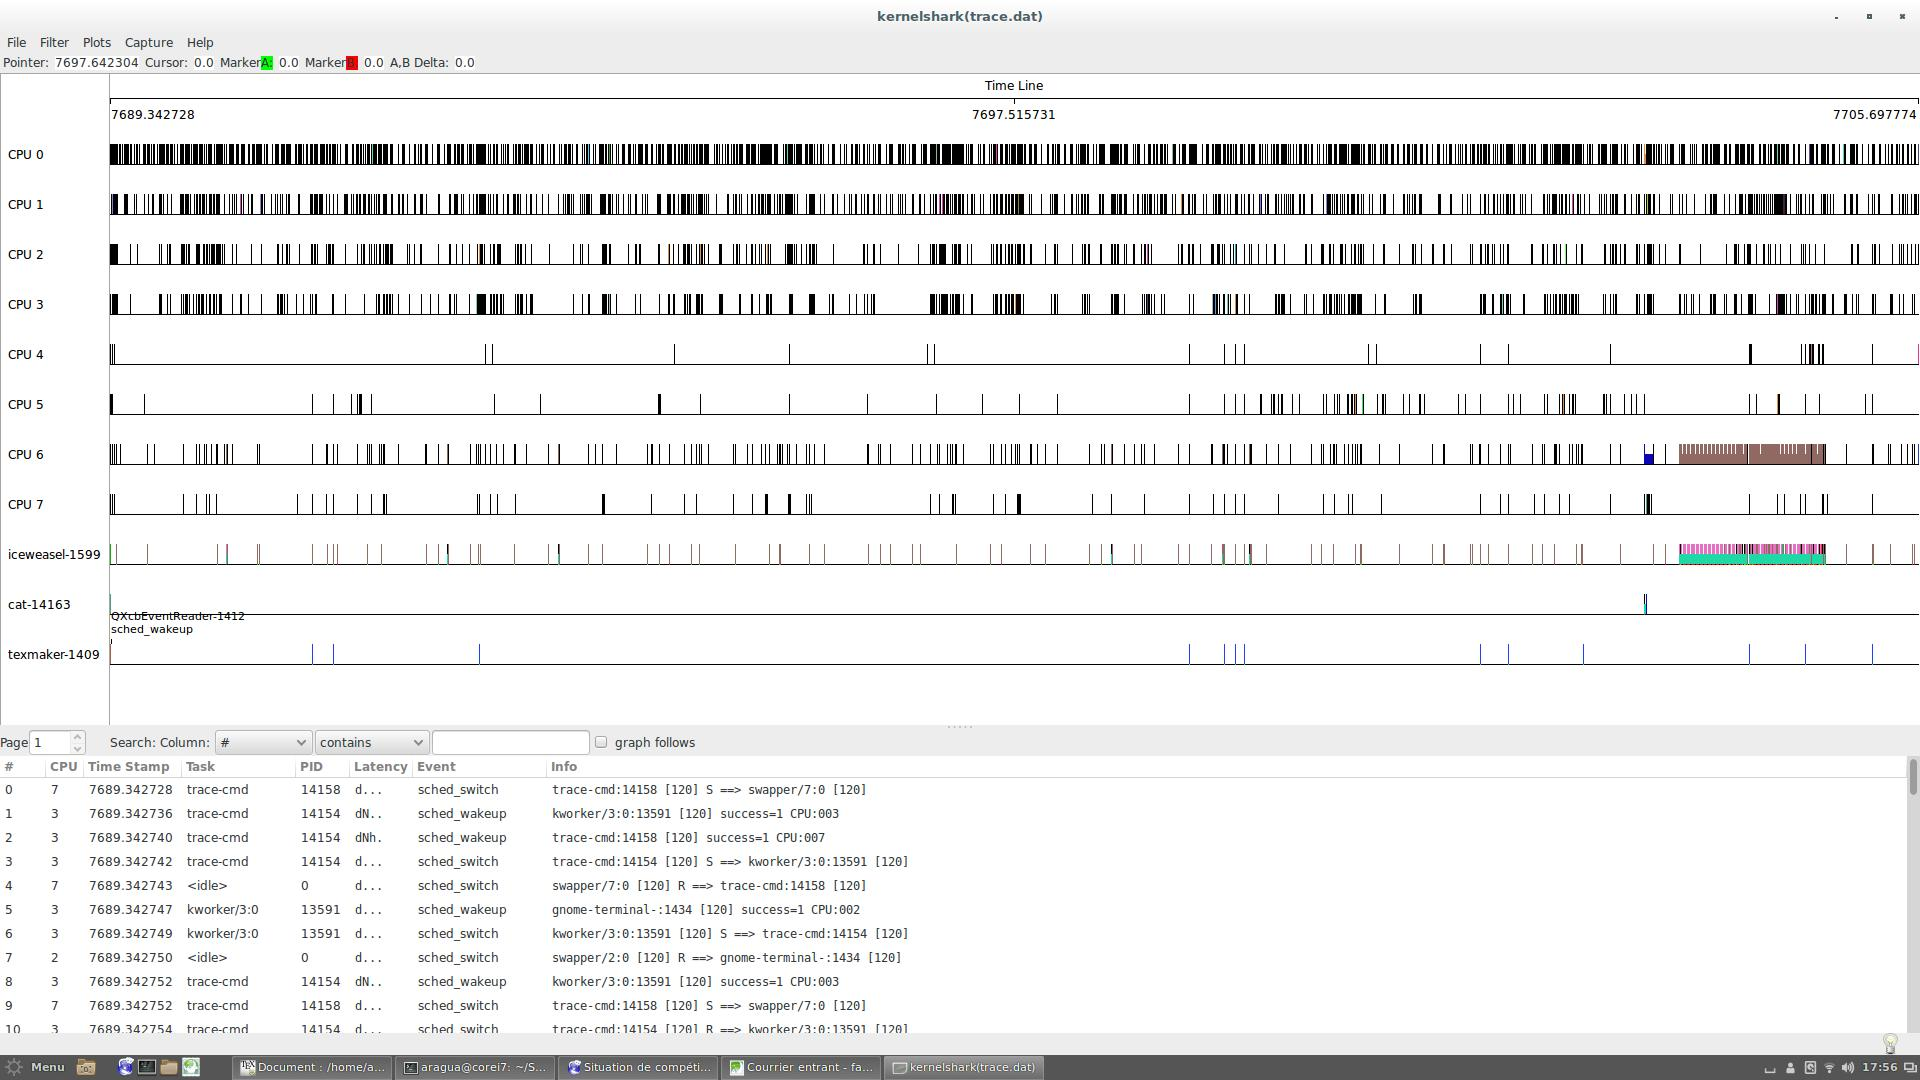
\includegraphics[width=11cm]{kernelshark.jpg}
\end{frame}



%%%%%%%%%%%%%%%%%%%%%%%    GOOD PRACTICES    %%%%%%%%%%%%%%%%%%%%%%%
\section{Bonnes pratiques}

\subsection{Eviter les bugs}
\begin{frame}{Éviter les bugs}
	\begin{itemize}
	 	\item
			Réfléchir avant d'agir
		\item
			Bien se documenter sur les fonctions, APIs utilisées
		\item
			Écrire du code simple, clair et modulaire
	 	\item
			Procéder étape par étape (ne pas tout coder d'un coup)			
	 	\item
			Vérifier les paramètres d'entrées dès que nécessaire
	 	\item
			Bien vérifier alloc, free, lock, unlock, ...
	 	\item
			Respecter les guidelines (Linux)
	\end{itemize}
\end{frame}

\subsection{Faciliter l'analyse}
\begin{frame}{Faciliter l'analyse}
	\begin{itemize}
	 	\item
			Utilisation de printf, zlog, syslog, printk, ftrace ...
		\item
			Utilisation de /proc ou d'un outil de stats en userland
		\item
			Wrapper des fonctions systèmes sensibles alloc, mutex, ... (facilite l'ajout de trace)
		\item
			Utiliser les mécanismes existants (stack-protector, timeout lock, RCU debug, ...)
	\end{itemize}
\end{frame}


%%%%%%%%%%%%%%%%%%%%%%%    En résumé    %%%%%%%%%%%%%%%%%%%%%%%
\section{Conclusion}

\begin{frame}{Conclusion}
	\begin{itemize}
		\item
			Différents cas de bug et d'erreurs (parfois entremêlés)
		\item
			De nombreux outils et moyens de debugs (gdb, valgrind, lttng, trace ...)
		\item
			Pas de recette magique pour analyser un bug
		\item
			Bonne connaissance du système et des outils
		\item
			Savoir s'adapter à la situation
	\end{itemize}
\end{frame}

\begin{frame}{Fin}
\begin{center}
\huge{Merci.\\Questions?}
\end{center}
\end{frame}


%%%%%%%%%%%%%%%%%%%%%%%%    APPENDIX    %%%%%%%%%%%%%%%%%%%%%%%
% All of the following is optional and typically not needed. 
\appendix
\section<presentation>*{\appendixname}
\subsection<presentation>*{For Further Reading}

\begin{frame}[allowframebreaks]
  
    
  \begin{thebibliography}{10}
    
  \beamertemplatebookbibitems
  % Start with overview books.

  \bibitem{procfs}
	\hyperlink{cible}{aller `a la cible}
    A.~Author.
    \newblock {\em http://people.ee.ethz.ch/~arkeller/linux/multi/kernel\_user\_space\_howto-2.html\#ss2.2}.
    \newblock Some Press, 1990.
 
    
  \beamertemplatearticlebibitems
  % Followed by interesting articles. Keep the list short. 

  \bibitem{Someone2000}
    S.~Someone.
    \newblock On this and that.
    \newblock {\em Journal of This and That}, 2(1):50--100,
    2000.
  \end{thebibliography}
\end{frame}


%\begin{frame}
%\begin{thebibliography}{9}
%\setbeamertemplate{bibliography item}[online]
%\bibitem{A} ItemA
%\setbeamertemplate{bibliography item}[book]
%\bibitem{B} ItemB
%\setbeamertemplate{bibliography item}[article]
%\bibitem{C} ItemC
%\setbeamertemplate{bibliography item}[triangle]
%\bibitem{D} ItemD
%\setbeamertemplate{bibliography item}[text]
%\bibitem{E} ItemE
%\end{thebibliography}
%\end{frame}

\end{document}
